\section{Deskripsi Persoalan}
Terdapat sebuah \textit{marble rolling toy} seperti pada gambar berikut :
\begin{figure}[h!]
  \centering
  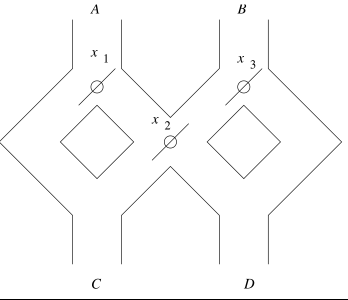
\includegraphics[width=250pt]{gambar.png}
  \caption{Ilustrasi \textit{Marble Rolling Toy}}
\end{figure}

\textit{Marble} akan digelindingkan dari A atau B. Ketika mengenai penghalang ($x_1, x_2, x_3$), \textit{marble} akan diarahkan sesuai penghalang tersebut. Lalu, penghalang yang dilalui \textit{marble} akan berganti arah. Jika \textit{marble} keluar di D, maka permainan dianggap berhasil. Mula-mula, semua penghalang menghadap ke kiri.

Permasalahan di atas ditranslasikan sebagai permasalahan DFA. Lalu, harus dibuat sebuah program dalam bahasa C atau Pascal yang memproses permasalahan DFA yang definisinya ada di sebuah file eksternal, lalu mengetes apakah string masukan pengguna diterima oleh DFA atau tidak. Program DFA itu akan digunakan untuk mengetes pada persoalan \textit{Marble Rolling Toy} apakah \textit{marble} terakhir masukan pengguna keluar di D atau tidak.
